\documentclass[12pt]{article}
%\usepackage{scicite}
\usepackage{times}
\usepackage{hyperref}
\usepackage{setspace}
\usepackage{amsmath}
\usepackage{listings}
\usepackage{graphicx}


\makeatletter
\renewcommand*\env@matrix[1][*\c@MaxMatrixCols c]{%
  \hskip -\arraycolsep
  \let\@ifnextchar\new@ifnextchar
  \array{#1}}
\makeatother

\topmargin 0.0cm
\oddsidemargin 0.2cm
\textwidth 16cm 
\textheight 21cm
\footskip 1.0cm

%The next command sets up an environment for the abstract to your paper.

\newenvironment{sciabstract}{%
\begin{quote} \bf}
{\end{quote}}


% If your reference list includes text notes as well as references,
% include the following line; otherwise, comment it out.

%\renewcommand\refname{References}

% The following lines set up an environment for the last note in the
% reference list, which commonly includes acknowledgments of funding,
% help, etc.  It's intended for users of BibTeX or the {thebibliography}
% environment.  Users who are hand-coding their references at the end
% using a list environment such as {enumerate} can simply add another
% item at the end, and it will be numbered automatically.




% Include your paper's title here

\title{FYS4150 Project 1} 
\author
{Mikkel Killingmoe Christensen\\
\\
\normalsize{\today}
}

% Include the date command, but leave its argument blank.

\date{}
%%%%%%%%%%%%%%%%% END OF PREAMBLE %%%%%%%%%%%%%%%%



\begin{document} 

% Double-space the manuscript.

\baselineskip24pt

% Make the title.

\maketitle 



% Place your abstract within the special {sciabstract} environment.

\begin{center}
{\large \textbf{Abstract}}
\end{center}
\begin{sciabstract}
Insert  Abstract here
\end{sciabstract}

\par GitHub repository:
\par \url{https://github.com/mikkello/FYS4150/}

\section{Introduction}
In this project, the goal is to find a numerical solution to a second degree differential equation. An example of such an equation is Poisson's equation in electromagnetism given by:
\begin{equation}
\frac{d^{2} \phi}{dr^{2}}=-4 \pi r\rho (r)
\end{equation}

This type of differential equation can be rewritten as the following with Dirichlet boundary conditions:
\begin{equation}
-u^{''}(x)=f(x), \quad x\in(0,1), \quad u(0)=u(1)=0
\end{equation}



\section{Theory}
\subsection{Poisson equation}
To solve the one-dimensional Poisson equation with Dirchelet boundary conditions, an approximation of the second derivative is made using Taylor expansion:
\begin{equation}
\frac{d^{2}u}{dx^{2}}\approx\frac{u(x+h)+u(x-h)-2u(x)}{h^{2}}+O(h^{2})
\end{equation}
where $O(h^{2})$ is the truncation error. 

The equation is then discretized and a simpler notation is used to yield the following:

\begin{equation}
\frac{u_{i+1}+u_{i-1}-2u_{i}}{h^{2}}=-f_{i}
\end{equation}

The step size is given by:
\begin{equation}
h = \frac{1}{n+1}
\end{equation}

Furthermore, the equation is a system of linear equations and can thus be written as a linear equation using linear algebra. The equation reads as follows:
\begin{equation}
\mathbf{A}u=h^{2}\mathbf{f}
\end{equation}
with
\begin{equation}
\mathbf{A} = \begin{bmatrix}
                           2& -1& 0 &\dots   & \dots &0 \\
                           -1 & 2 & -1 &0 &\dots &\dots \\
                           0&-1 &2 & -1 & 0 & \dots \\
                           & \dots   & \dots &\dots   &\dots & \dots \\
                           0&\dots   &  &-1 &2& -1 \\
                           0&\dots    &  & 0  &-1 & 2 \\
                      \end{bmatrix}
                      \label{eq:tridiagm}
\end{equation}
being a tridiagonal  $n\times n$ matrix. The problem is now possible to solve by finding the vector $\mathbf{u}$. For small matrices, this can easily be done by multiplying both sides with the inverse of $\mathbf{A}$. For larger matrices, however, this procedures is very slow and a better method is needed. 

\subsubsection{Analytical solution}
Analytical solutions exists for the Poisson equation problem, and it will be useful to compare this to the numerical results. 
For the term:
\begin{equation}
f(x) = 100e^{-10x}
\end{equation}
the exact solution is:
\begin{equation}
u(x) = 1-(1-e^{-10})x-e^{-10x}
\end{equation}

\subsection{Guassian elimination}
Guassian elimination is an efficient method for solving these types of equations. The matrix is here transformed into the identity matrix, while a new vector $\tilde{d}$ is created with the solution. 

The elimination is here shown with a generalized 4x4 matrix, but the method works for any $n\times n$ matrix. 

\begin{equation}
\begin{bmatrix}
                           a_{1}&b_{1}&0&0 \\
                           c_{1}&a_{2}&b_{2}&0\\
                           0&c_{2}&a_{3}&b_{3}\\
                           0&0&c_{3}&a_{4}
                      \end{bmatrix}
                      \begin{bmatrix}
                           u_{1} \\
                           u_{2}\\
                           u_{3}\\
                           u_{4}
                      \end{bmatrix}
                      =
                      \begin{bmatrix}
                           d_{1} \\
                           d_{2}\\
                           d_{3}\\
                           d_{4}
                      \end{bmatrix}
\end{equation}
\subsubsection{Forward substitution}
To remove the elements below the diagonal in the matrix, the method of forward substitution is used. The first operation is to subtract $\frac{c_{1}}{a_{1}}$ times the first row. 
This will create an extended matrix looking like this: 
\begin{equation}
\begin{bmatrix}[cccc|c]
                           a_{1}&b_{1}&0&0& d_{1}\\
                           c_{1}&a_{2}&b_{2}&0& d_{2}\\
                           0&c_{2}&a_{3}&b_{3}& d_{3}\\
                           0&0&c_{3}&a_{4}& d_{4}
                      \end{bmatrix}
                      \sim
                      \begin{bmatrix}[cccc|c]
                           a_{1}&b_{1}&0&0& d_{1}\\
                           0&a_{2}-\frac{c_{1}b_{1}}{a_{1}}&b_{2}&0& d_{2}-\frac{d_{1}c_{1}}{a_{1}}\\
                           0&c_{2}&a_{3}&b_{3}& d_{3}\\
                           0&0&c_{3}&a_{4}& d_{4}
\end{bmatrix}
\end{equation}
These operations can be generalized by introducing the new variables
\begin{equation}
\tilde{a}_{i}=a_{i}-\frac{b_{i-1}c_{i-1}}{\tilde{a}_{i-1}}
\end{equation}
\begin{equation}
\tilde{d}_{i}=d_{i}-\frac{\tilde{d}_{i-1}c_{i-1}}{\tilde{a}_{i-1}}
\end{equation}
Continuing the row reduction with the forward substitution starting with the lowest index of the c-diagonal will yield the following equation:

\begin{equation}
\begin{bmatrix}
                           \tilde{a}_{1}&b_{1}&0&0\\
                           0&\tilde{a}_{2}&b_{2}&0\\
                           0&0&\tilde{a}_{3}&b_{3}\\
                           0&0&0&\tilde{a}_{4}
                      \end{bmatrix}
                      \begin{bmatrix}
                           u_{1} \\
                           u_{2}\\
                           u_{3}\\
                           u_{4}
                      \end{bmatrix}
                      =
                      \begin{bmatrix}
                           \tilde{d}_{1} \\
                           \tilde{d}_{2}\\
                           \tilde{d}_{3}\\
                           \tilde{d}_{4}
                      \end{bmatrix}
\end{equation}
with the boundary conditions $\tilde{a}_{1}=a_{1}$ and $\tilde{d}_{1}=d_{1}$

The two formulas in the forwards substitution requires three floating point operations each, yielding a total of $6(n-1)$ FLOPS.
\subsubsection{Backward substitution}
To remove the elements above the diagonal in the matrix, the method of backward substitution is used. As opposed to the forward substitution, we start with the highest index of the b-diagonal. The first operation is to remove $b_{3}$ by subtracting the third row with $\frac{b_{3}}{\tilde{a}_{4}}$ times the fourth row. 

\begin{equation}
\begin{bmatrix}[cccc|c]
                           \tilde{a}_{1}&b_{1}&0&0&\tilde{d}_{1}\\
                           0&\tilde{a}_{2}&b_{2}&0&\tilde{d}_{2}\\
                           0&0&\tilde{a}_{3}&b_{3}&\tilde{d}_{3}\\
                           0&0&0&\tilde{a}_{4}&\tilde{d}_{4}
                      \end{bmatrix}
                      \sim
                      \begin{bmatrix}[cccc|c]
                           \tilde{a}_{1}&b_{1}&0&0& \tilde{d}_{1}\\
                           0&\tilde{a}_{2}&b_{2}&0& \tilde{d}_{2}\\
                           0&0&\tilde{a}_{3}&0& \tilde{d}_{3}-\frac{b_{3}\tilde{d}_{4}}{\tilde{a}_{4}}\\
                           0&0&0&\tilde{a}_{4}& \tilde{d}_{4}
                      \end{bmatrix}
\end{equation}
Repeating the procedure on the other rows will remove $b_{2}$ and $b_{3}$ and yield the following matrix:
\begin{equation}
\begin{bmatrix}[cccc|c]
\tilde{a}_{1}&0&0&0&\tilde{d}_{1}-\frac{b_{1}}{\tilde{a}_{3}}(\tilde{d}_{2}-\frac{b_{2}}{\tilde{a}_{3}}(\tilde{d}_{3}-\frac{b_{3}\tilde{d}_{4}}{\tilde{a}_{4}})) \\
0&\tilde{a}_{2}&0&0&\tilde{d}_{2}-\frac{b_{2}}{\tilde{a}_{3}}(\tilde{d}_{3}-\frac{b_{3}\tilde{d}_{4}}{\tilde{a}_{4}})\\
0&0&\tilde{a}_{3}&0&\tilde{d}_{3}-\frac{b_{3}\tilde{d}_{4}}{\tilde{a}_{4}}\\
0&0&0&\tilde{a}_{4}&\tilde{d}_{4}

\end{bmatrix}
\end{equation}
Putting this new matrix into the linear equation, the following relations can be found:
\begin{equation}
u_{4}=\frac{\tilde{d}_{4}}{\tilde{a}_{4}}
\end{equation}
and
\begin{equation}
u_{3}=\frac{\tilde{d}_{3}-b_{3}u_{4}}{\tilde{a}_{3}}
\end{equation}
Generalizing this to a matrix with i-rows, the following formula for $u_{i}$ can be found:
\begin{equation}
u_{i}=\frac{\tilde{d}_{i}-b_{i}u_{i+1}}{\tilde{a}_{i}}
\end{equation}
This formula requires three floating point operations, yielding a total of $3(n-1)$ FLOPS. This means that the full Guassian elimination requires $9(n-1)$ FLOPS. 


\subsubsection{Numerical implementation of the Gaussian elimination}

\lstset{language=Python}
\lstset{frame=lines}
\lstset{caption={Implementing the Gaussian elimination algorithms in Python}}
\lstset{label={lst:code_direct}}
\lstset{basicstyle=\footnotesize}
\begin{lstlisting}
from brg.datastructures import Mesh
 
mesh = Mesh.from_obj('faces.obj')
mesh.draw()
\end{lstlisting}

\subsubsection{Gaussian elimination of a tridiagonal matrix}
The fact that the matrix (\ref{eq:tridiagm}) that will be used in this problem is a tridiagonal matrix with two of the diagonals being $-1$, can simplify our algorithms and save some FLOPS.

Updating the Guassian elimination formulas with this special case, yields the following new equations:

\begin{equation}
\tilde{a}_{i}=\tilde{a}_{i}+\frac{b_{i-1}}{\tilde{a}_{i-1}}
\end{equation}
which can be further simplified to:
\begin{equation}
\tilde{a}_{i}=\frac{i}{i+1}
\label{eq:a_i}
\end{equation}
\begin{equation}
\tilde{d}_{i}=d_{i}+\frac{\tilde{d}_{i-1}}{\tilde{a}_{i-1}}
\end{equation}
\begin{equation}
u_{i}=\frac{\tilde{d}_{i}+u_{i+1}}{\tilde{a}_{i}}
\end{equation}

The new set of equations will require $4(n-1)$ FLOPS, which is a great reduction in the required computation power. Equation (\ref{eq:a_i}) can be pre-calculated outside the algorithm and will therefore not add more FLOPS.

\subsubsection{Numerical implementation of the special case}
\lstset{language=Python}
\lstset{frame=lines}
\lstset{caption={Implementing the Gaussian elimination algorithms in Python for the special case}}
\lstset{label={lst:code_direct}}
\lstset{basicstyle=\footnotesize}
\begin{lstlisting}
from brg.datastructures import Mesh
 
mesh = Mesh.from_obj('faces.obj')
mesh.draw()
\end{lstlisting}

\subsection{LU-decomposition}
Decomposing a matrix in one lower triagonal and one upper triagonal matrix is called LU-decomposition. This can be done to split a matrix equation into to new equations which makes the problem easier to solve. 
The matrix equation $A\mathbf{u}=\mathbf{v}$ will then read:
\begin{equation}
LU\mathbf{u}=\mathbf{v}
\end{equation}
After introducing $\mathbf{y}=U\mathbf{u}$, the solution can be computed. First $\mathbf{y}$ is found from:
\begin{equation}
L\mathbf{y}=\mathbf{v}
\end{equation}
Then, \begin{equation}
U\mathbf{u}=y
\end{equation}
can be solved to find $\mathbf{u}$. 

\section{Method and results}
\subsection{Plot of the analytical solution}
The analytical solution was plotted to get a feeling of what the numerical solution would look like. It can be seen in figure (\ref{fig:analytical}).

\begin{figure}
\caption{Analytical solution}
\label{fig:analytical}
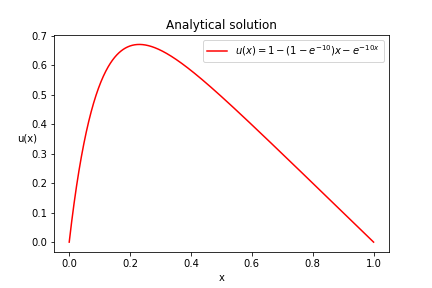
\includegraphics[]{analytical.png}
\end{figure}

\subsection{Implementation of general solver}
A Python-program for the general solver was made, and the second derivative for $f(x)=100e^{-10x}$ was calculated and compared with the analytical results for $n = 10, 100, 1000$. The calculation times were calculated and can be found in table (\ref{tab:general}).


\begin{table}[]
\centering
\caption{My caption}
\label{tab:general}
\begin{tabular}{|l|l|l|l|l|}
\hline
n    & General & Special & LU &  \\ \hline
10   &         &         &    &  \\ \hline
100  &         &         &    &  \\ \hline
1000 &         &         &    &  \\ \hline
\end{tabular}
\end{table}

\section{Discussion and conclusion}
















%-----------------------------------------------------%



\begin{flushleft}

\begin{thebibliography}{}

\singlespacing
\small




  
\bibitem{Article}
  Morten Hjorth-Jensen,
  Computational Physics,
  August 2015
  
\end{thebibliography}
\end{flushleft}






\end{document}




















